
\documentclass[a4paper,12pt]{article}
\usepackage{epstopdf}
\usepackage[utf8]{inputenc}
\usepackage[swedish]{babel}
\usepackage{enumerate}
\usepackage{mathtools}
\usepackage{hyperref}
\usepackage{float}
\usepackage[pdftex]{graphicx}   
\usepackage{multirow}
\usepackage{listings}
\lstset{
    language=R,
    basicstyle=\ttfamily
}

\title{TDDE01 -- Machine Learning \\
       Individual Laboration Report 2}
\author{Martin Estgren \texttt{<mares480>}}
      
\begin{document}
 \pagenumbering{arabic}
    \maketitle % Generate.
\section{Assignment 1}

In this assignment we were tasked with implementing \textit{feature selection} using the \textit{k-fold cross validation} and \textit{linear regression} algorithms. The result of this can be found in appendix: A - Code assignment 1. 

The feature selection algorithm iterates through all possible combinations of \textit{features} from the predictor variables and apply the \textit{k-fold} cross validation on all of them. The feature combination with the lowest \textit{sum of squared error} gets picked as the best combination. 
\begin{equation}
  \mathbf{A} = \{c_1,c_2,...,c_n\}, 1 \le n \le ncol(X)
\end{equation} 
\( \mathbf{A} \) in the equation above represents all the permutations of column index for the response variable. Each of theses combinations are sent to the \textit{k-fold cross validation} where the data is split into  \( \mathit{K} \)  parts of equal size. The  \( \mathit{K} \) are then iterated through and each data subset is used as testing data with the other \( \mathit{K} -1 \) sets as training data. The \textit{k-fold cross validation} uses the \textit{linear regression} with \textit{ordinary least squares} estimator.  The produced predictions are then error checked with the \textit{sum of squared error} 
\begin{equation}
  \sum _{i = 1} ^{n} (\hat{y}_i - y_i), n = nrow(y)
\end{equation} 
for fold \( \mathit{K} \). After all the \( \mathit{K} \) folds for a given combination of features are calculated, the mean of all fold errors are calculated and returned as the final error value for the feature combination.
\begin{equation}
\frac{1}{\mathit{K}}\sum_{k = 1}^{\mathit{K}} ( \sum _{i = 1} ^{n} (\hat{y}_i - y_i))
\end{equation} 
where \( \mathit{K} = |folds|\) and \(n = |y|\).

In the figure below the mean error for a given number of selected features can be shown. 

\begin{figure}[H]
\centering
\begin{minipage}[]{0.5\textwidth}
  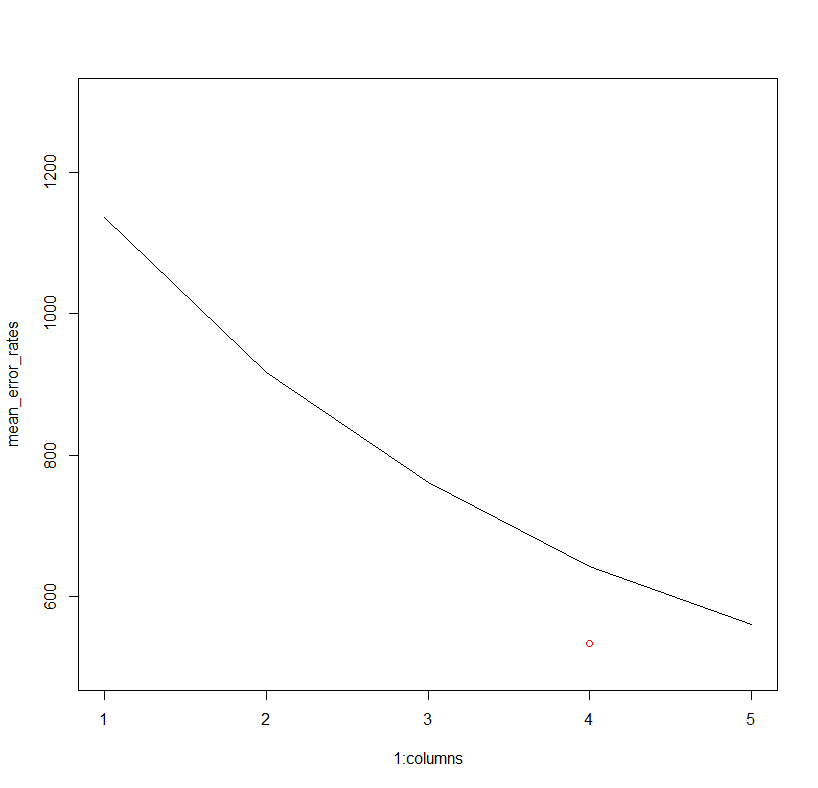
\includegraphics[width=\textwidth]{figures/Lab2A1_me_features.png}  
  \caption{The mean error rate for different number of feature combinations.\label{fig:features} }
 \end{minipage}
\end{figure}

The red dot indicates the best feature combination, i.e. the one with the lowest error score. For this data set it's \( \{Agriculture, Education, Catholic, Infant.Mortality\} \). In general terms we can observe that the more features that are selected, the lower the error rate becomes.

The following graphs show the linear regression result for each of the different features that was returned by the best feature subset function described above.

\begin{figure}[H]
\centering
\begin{minipage}[]{0.24\textwidth}
  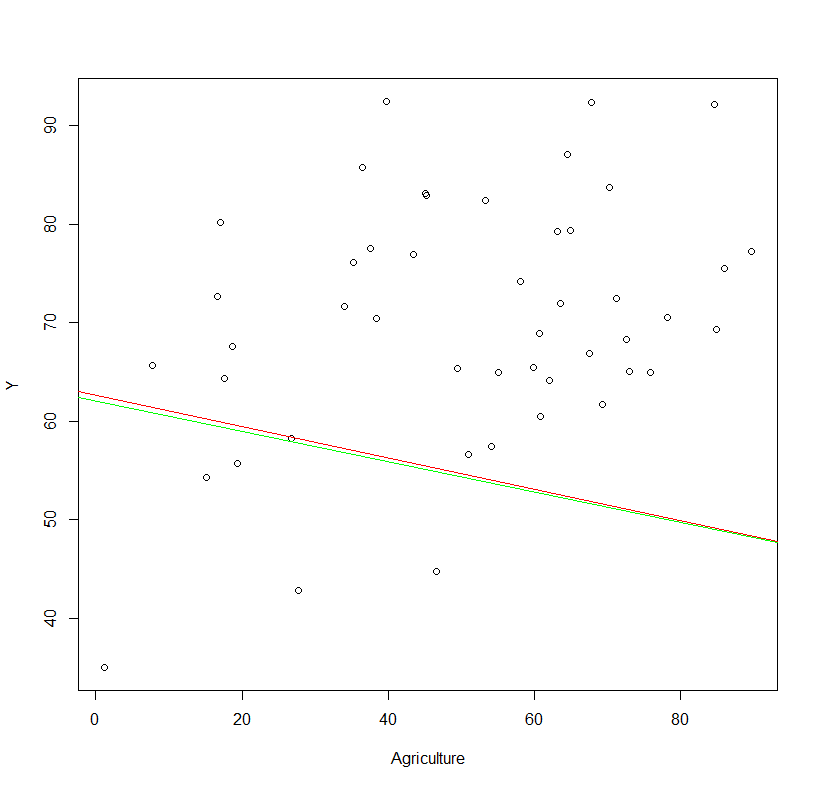
\includegraphics[width=\textwidth]{figures/Lab2A1_lr_A.png}  
 \end{minipage}
 \begin{minipage}[]{0.24\textwidth}
  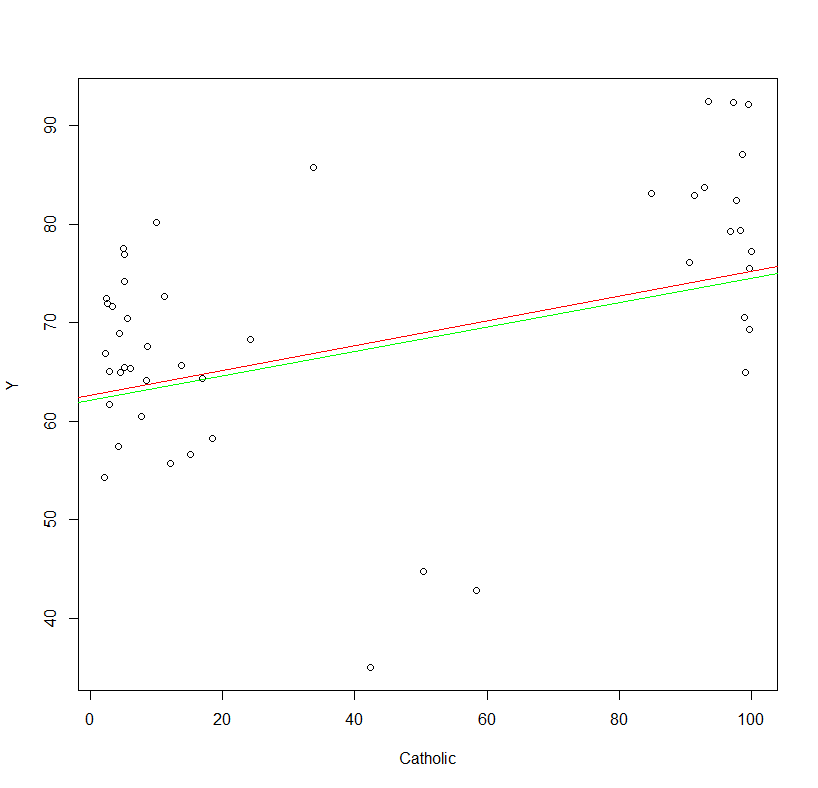
\includegraphics[width=\textwidth]{figures/Lab2A1_lr_C.png}  
 \end{minipage}
 \begin{minipage}[]{0.24\textwidth}
  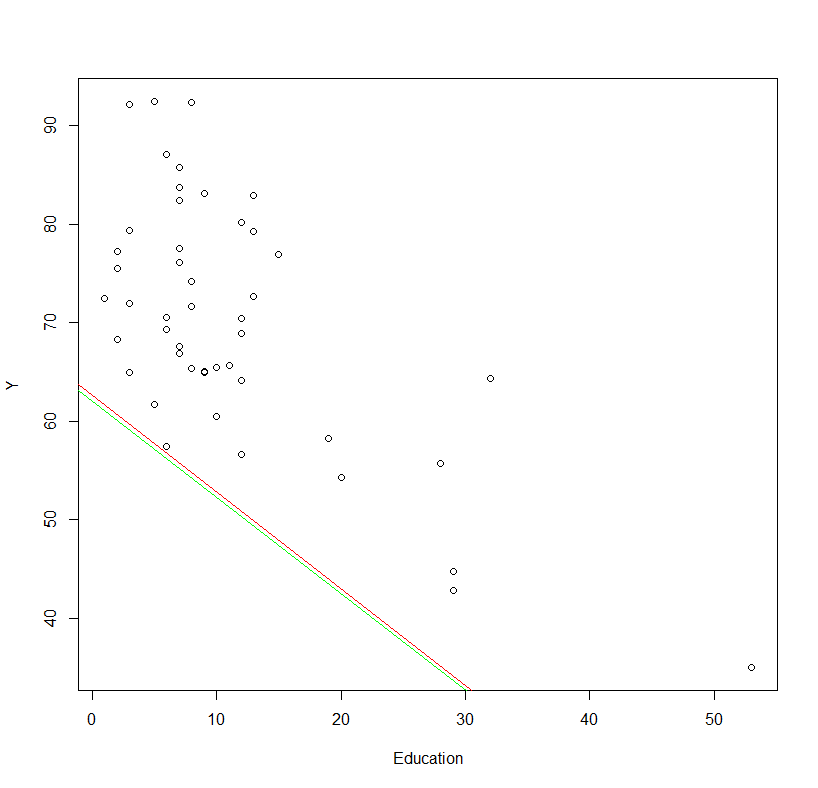
\includegraphics[width=\textwidth]{figures/Lab2A1_lr_E.png}  
 \end{minipage}
 \begin{minipage}[]{0.24\textwidth}
  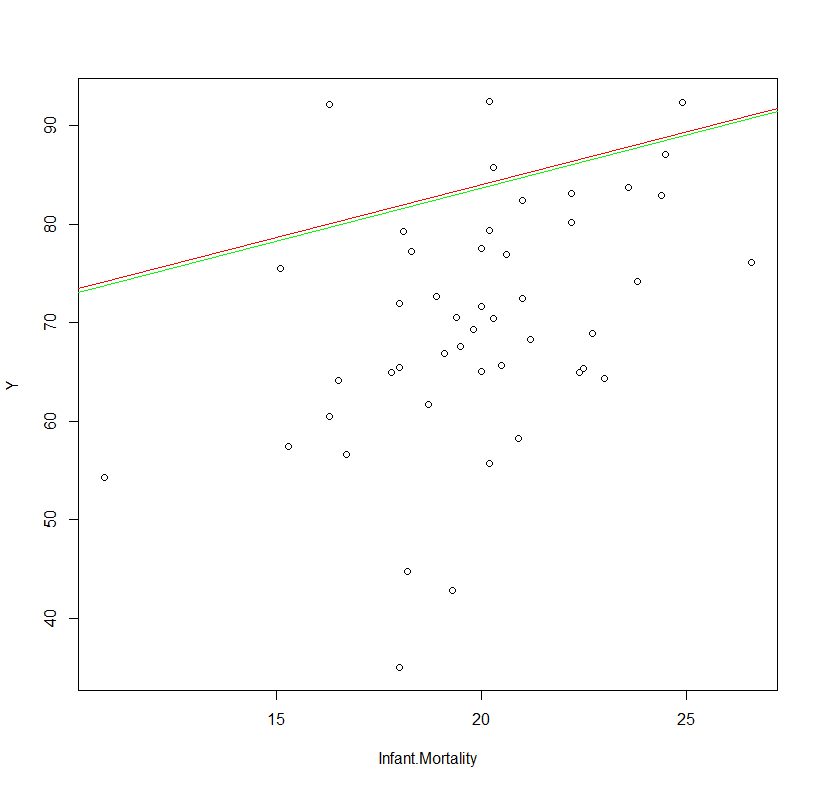
\includegraphics[width=\textwidth]{figures/lab2A1_lr_IM.png}  
 \end{minipage}
\end{figure}

The models aren't perfect but manges to hit fairly close to what humans would recognize as the best linear function for each data set.

\section{Assignment 2}

In this assignment we are tasked with analyzing the data set found in the file \textbf{tecator.xlsx}. The data is grouped into the columns: \( \{ Sample, Channel 1, ... , Channel 100, Moisutre, Fat, Protein \} \). The first task is to plot the \textit{Moisture} and \textit{Protein} and determine if a linear model would be a good approximation for the data. The plot can be seen in the figure below.

\begin{figure}[H]
\centering
\begin{minipage}[]{0.5\textwidth}
  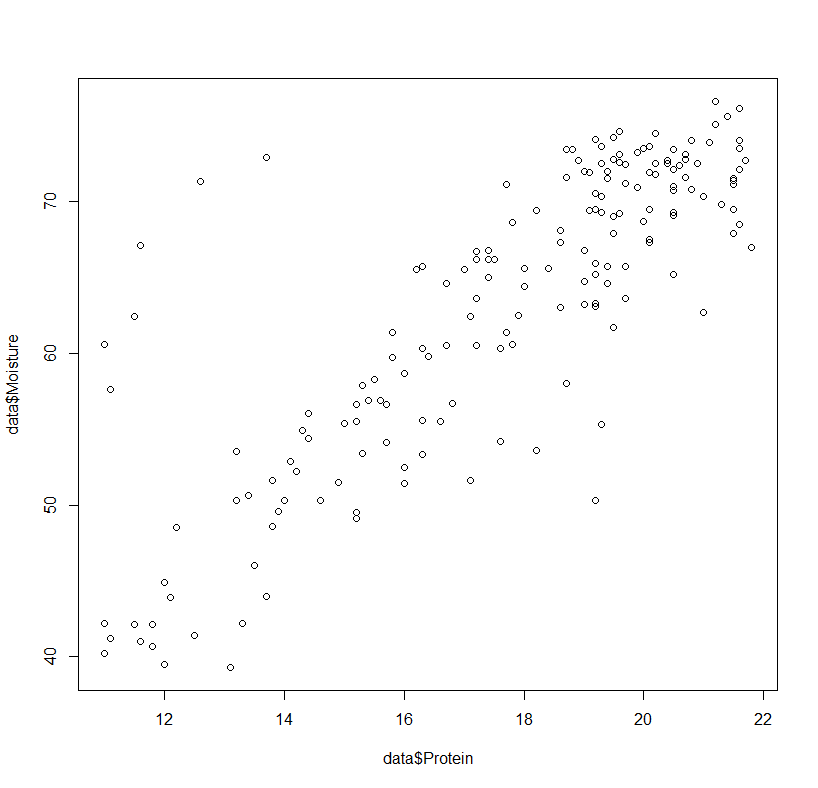
\includegraphics[width=\textwidth]{figures/Lab2A2_data_plot.png}  
  \caption{The \textit{Moisture} plotted by \textit{Protein}.\label{fig:data plot} }
 \end{minipage}
\end{figure}

A linear approximation seems to be a good fit for the data.

Next we examine if a polynomial approximation of the data up to the \(n\)th power and using \textit{mean squared error} (MSE) to examine the fitness of the polynomial model. The data set is split into two sets of equal size where one of the sets are the training set and the other the validation set. 

\begin{figure}[H]
\centering
\begin{minipage}[]{0.75\textwidth}
  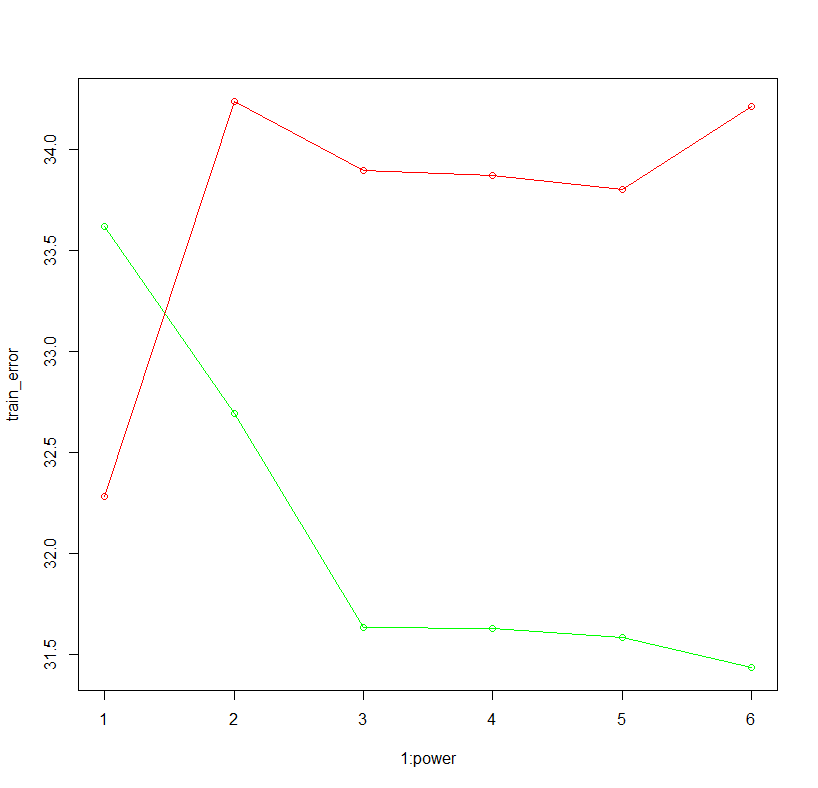
\includegraphics[width=\textwidth]{figures/Lab2A2_test_train_err.png}  
  \caption{The training and validation error rate for the polynomial estimation given the MSE.}
 \end{minipage}
\end{figure}

The \textbf{green line} is the error rate for the training data and the \textbf{red line} is the error rate for the validation set over the different power-levels. We can observe in the graph that the fitting of the training data decreases when the power-level increases but the error rate for the validation data increases with about the same magnitude. This can be explained with the fact that, as observed in the plot of the full data set above, the data would follow a linear model and the polynomial approximation leads to over fitting of the training set.  


\textbf{T.B.C}
The next part involves performing variable selection on the full data set with the \textit{step} variable selection function. We get 64 coefficients form the step function.

The next part involves fitting a ridge regression model to the data set . The result can be observed in the following plot. We can see as the lambda increases, the coefficients converges to zero.

The lasso regression model results in fewer coefficients and less more non continuous coefficient functions over the lambdas. 

The final part involves plotting to cross validation score using the lasso model, the result can be observed in the graph below. The variance increase with the lambda and the validation score  

In comparison with the step aic model the cross validation using lasso and k-fold resulted in much less coefficients. 


\section{Appendix: A - Code assignment 1}

\lstinputlisting[caption=Code for assignment 1,
    label={code/assignment1.r},
    breaklines=true]
    {code/assignment1.r}

\section{Appendix: B - Code assignment 2}

\lstinputlisting[caption=Code for assignment2 ,
    label={code/assignment2.r},
    breaklines=true]
    {code/assignment2.r}
\end{document}
